\chapter{基于自然语言处理模型的文件访问模式识别}
自然语言处理(NLP)的定义可以简单概括对人类语言进行自动化、智能化分析以及学会人类表达的一系列计算机技术,是一门包含着计算机科学、时间序列分析以及语言学的交叉学科,这些学科既有区别又相互交叉。

1936年A.M.Turing发明了举世闻名的“图灵机”,使数学中的逻辑符号和真实世界之间建立了联系,为后来计算机的蓬勃发展提供了坚实的理论基础。20世纪50年代,在图灵机的计算模型的基础上,自动机理论被提出,是现代计算机科学发展的基础\cite{自然语言处理的历史与现状}。后来Kleene又在自动机理论模型之基础上提出了正则表达式和有限自动机。1956年,Chomsky提出了上下文无关的语法的理论,同年人工智能被发明后,被迅速应用到自然语言处理领域之中。上下文无关语法的提出使得该领域的研究分为了基于推理规则的符号派和基于概率论的随机派\cite{宋一凡2019自然语言处理的发展历史与现状},在之后很多年里分别高速发展。70年代语音识别算法研制成功,隐马尔科夫模型(Hidden Markov Model,HMM)提出并得到了广泛应用\cite{自然语言处理的历史与现状}。

近年来,随着深度学习的飞速发展,自然语言处理领域也取得了诸多重要突破。RonanCollobert等\cite{Natural_language_processing_(almost)_from_scratch}于2011年的研究提出了一个简单的深度学习框架,在许多NLP经典任务中取得了前所未有的性能,如实体命名识别、语义标注和词性标注等。之后,研究人员提出了大量基于复杂深度学习的算法,用于解决有难度的NLP任务。2013年,Mikolv\cite{skipgram}提出了当前NLP领域最重要的模型之一Skip-gram,该模型以出色的性能表现将单词转化为高维向量,为后续如雨后春笋般涌现的自然语言处理模型奠定了基础。

本章后续内容以词嵌入方法、循环神经网络等主流自然语言处理模型为基础,探讨其在文件系统优化,尤其是数据迁移策略中“冷”、“热”文件分类问题的应用。

\section{基于词嵌入模型的文件名向量化}
\subsection{词嵌入方法概述}

\href{https://www.linkresearcher.com/careers/6c7a15b5-236a-40f3-879f-af2ac06c2557}{NLP综述博客}
\href{https://blog.csdn.net/mawenqi0729/article/details/80698350}{词嵌入博客}

众所周知,在自然语言处理任务中,第一步工作就是用计算机能够理解的方式表示和描述单词,也就是将其用向量表示。通常有两大类表征方式:离散型表示(one-hot)和分布型表示(distributed representation)。

所谓离散型表示是指,在给定词汇表$V$的条件下,每一个单词被表示为一个维度为$|V|$的向量,该词汇表中任意一个单词,唯一地分配一个维度为1,其余维度均为0。例如单词file在词汇表中第二个出现,则其离散型向量表示为:$v_{file} = [0,1,0,\dots,0]$。这种表示方式相当于为每个单词分配了一个唯一的ID。当词汇表较大时,词嵌入的维度将会非常高,并且无法表达词与词之间的关系。

单词的分布式表示基于语义学中的分布式假设(Distributional Hypothesis)\cite{distributional_hypothesis}:
在相似的上下文中出现的单词通常具有相似的含义。例如单词water和coffee常与drink搭配,因此water与coffee具备一定的的相似性。分布式表示的目的就是将单词转化为稠密的向量(与离散型的one-hot向量相对),将人类自然语言中的单词之间的相似性和逻辑关联转化为向量空间的数学关系来处理(例如使用二范数表达单词的相似度)。见图\ref{fig:t_sne}所示例子,Li等人\cite{visualizing}采用t-SNE方法对60维的词嵌入进行降维处理,结果显示,含义相近的单词在向量空间内“距离”也比较接近。
\begin{figure}[htp]
\centering
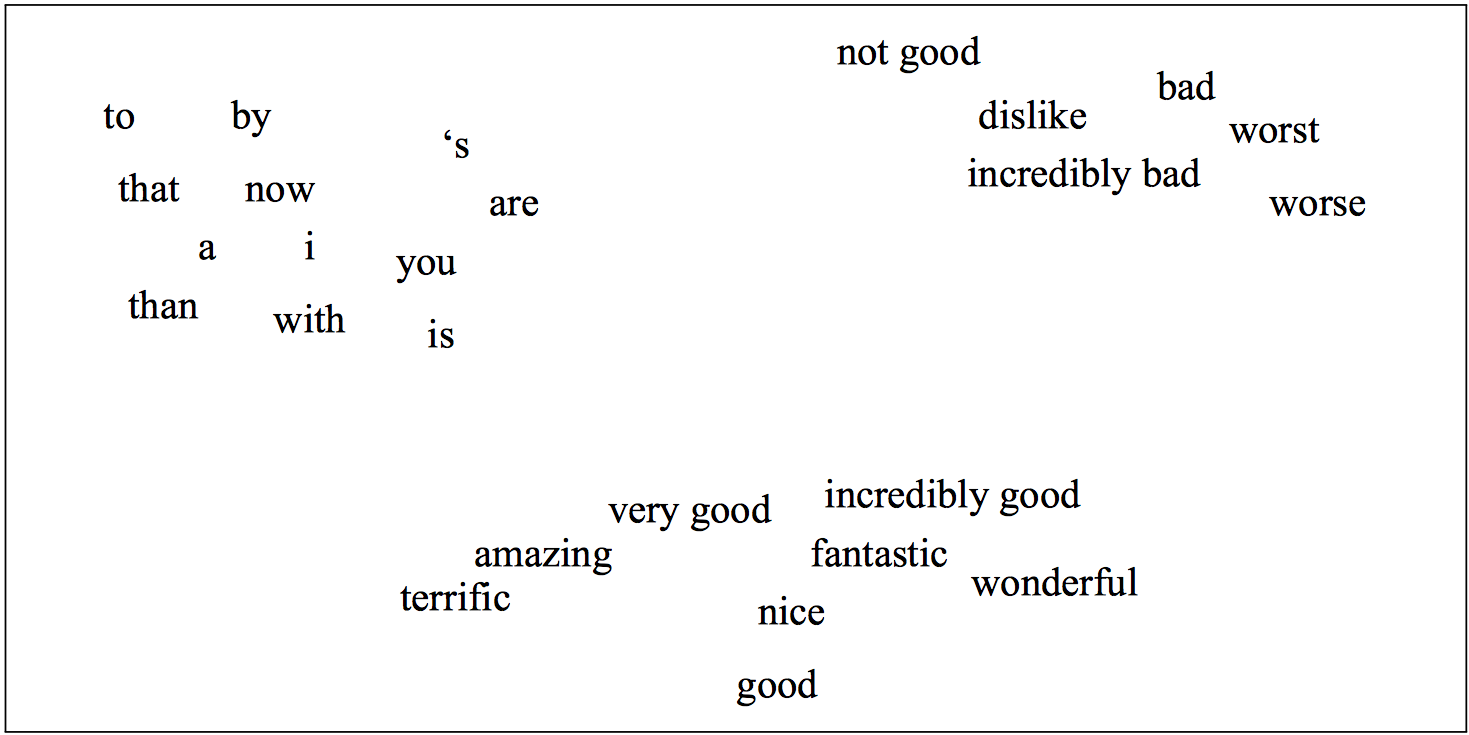
\includegraphics[width=\textwidth]{t_sne}
\caption{词向量降维后的可视化}
\label{fig:t_sne}
\end{figure}
{\color{red}词嵌入降维图}\linkout{nlp_book}{107}

{\color{red}词嵌入相关文献}\linkout{nlp_book}{128}

为实现这种从自然语言到向量空间的映射,自然语言处理发展历史上出现了许多理论和方法,例如Deerwester于1988年提出的潜在语义索引(Latent Semantic Indexing)方法\cite{LSI},以及该作者后续应用奇异值分解(SVD)对共现矩阵降维而实现的潜在语义分析方法(latent semantic analysis)\cite{LSA},在此后多年里被广泛应用于多种NLP任务,如认知模型\cite{cognitive_model},拼写检查\cite{spell_checking},写作评分\cite{essay_grading}等等。

随着近年来深度学习的发展,基于神经网络的自然语言模型开始流行,Bengio分别在2003年\cite{bengio2003}和2006年\cite{bengio2006}发表的成果表明,神经网络语言模型能在单词预测任务中出色地担任词嵌入转换的角色。

2013年,Mikolov提出了著名的连续词袋(CBOW)和Skip-gram模型\cite{skipgram},可以说这两种词嵌入模型的发明引发了NLP领域的深刻变革,至今为止这两种模型组成的Word2Vec方法仍被广泛使用于学术界和工业界。

\subsection{文件名、路径向量化}
在Unix文件系统中,任意文件或目录在被创建时,均会被分配一个唯一的ID,也就是Inode序号,以此作为唯一的标识以便于后续各种文件操作。Inode序号只与文件创建先后相关,是一种one-hot的表示方式。那么能否效仿自然语言处理中词嵌入的思想,建立一种能够包含文件或目录之间关联性的表征方式?

文件系统层次结构规范(Filesystem Hierarchy Standard,FHS)\cite{fhs}是由Linux基金会在1994年发起,旨在规范Linux各发行版和其他类Unix系统下文件目录结构的业界统一标准,至今已发展演变到FHS-3.0(2015年)。在FHS定义的目录结构规范下,Linux操作系统的目录组织结构和命名受到了明确严格的约束,例如:
\begin{itemize}
    \item /:根目录。
    \item /bin:系统执行文件目录。
    \item /boot:启动文件目录。
    \item /dev:驱动设备目录。
    \item /etc:系统配置文件目录。
    \item /lib, /usr/lib, /usr/local/lib:系统使用的函数库目录。
    \item ......
\end{itemize}

如果将一个文件的完整路径(如/usr/lib/python2.7/)视为一个句子,各级目录视为单词,我们假定上节提到的分布式假设同样成立,即:同一目录下的文件或目录具有类似的含义。直观上看,这个假设是合理的,例如/bin目录下的bash,rm,cp文件等均为可执行命令,/usr/lib/python2.7/目录下均为Python的库文件。在此假设成立的前提下,本节将介绍如何建立Skip-gram模型,对给定的Unix文件系统目录下所有文件名、目录名进行向量化。

\subsubsection*{语料库的生成}
众所周知,任何机器学习模型都离不开数据,自然语言处理领域的数据集通常被称为语料库(Corpus)。任何语言学的研究或者自然语言模型的建立都必须建立在大量的语料之上,否则无论是基于规则方法还是统计方法建立的模型都将失效。

为了建立文件路径相关的“语料库”,我们将从根目录(或文件系统的挂载点)开始,通过常规的遍历算法将此目录下所有文件、目录的完整路径逐行写入到一个文本文件,作为模型的训练数据集。
{\color{red}此处插入遍历算法}

\subsubsection*{Skip-gram模型建立}

\subsubsection*{模型训练与词向量生成}



\section{基于循环神经网络的文件访问模式分析}
\subsection{循环神经网络及其在时间序列分析中的应用}
\subsection{采用GRNN(Gated Recurrent Neural Network)的文件访问模式分析模型}
\section{本章小结}